\documentclass[10pt,twocolumn,letterpaper]{article}

\usepackage[margin=0.75in]{geometry}
\usepackage[utf8]{inputenc}
\usepackage[T1]{fontenc}
\usepackage{times}
\usepackage{graphicx}
\usepackage{amsmath}
\usepackage{amssymb}
\usepackage{booktabs}
\usepackage{multirow}
\usepackage{array}
\usepackage{xcolor}
\usepackage{url}
\usepackage[colorlinks=true,linkcolor=blue,citecolor=blue,urlcolor=blue]{hyperref}
\usepackage[numbers,sort&compress]{natbib}
\usepackage{caption}
\usepackage{float}
\usepackage{titlesec}

\setlength{\columnsep}{0.25in}
\setlength{\parskip}{0pt}
\setlength{\parindent}{1em}

\titleformat{\section}{\normalfont\large\bfseries}{\thesection.}{0.5em}{}
\titleformat{\subsection}{\normalfont\normalsize\bfseries}{\thesubsection.}{0.5em}{}

\graphicspath{{../figures/}}

\title{\vspace{-1em}\Large\bfseries Post-Execution Defect Attribution\\
via Fused Repository Priors and Failure Signals:\\
A Controlled Empirical Study on 6{,}000 Synthetic Failure Events}

\author{Vijay~P.~Javvadi\\
\textit{Independent Researcher}\\
\href{mailto:vijay@vijayjavvadiresearch.ai}{vijay@vijayjavvadiresearch.ai}\\
ORCID: \href{https://orcid.org/0009-0004-1192-6906}{0009-0004-1192-6906}\\
\url{https://vijayjavvadiresearch.ai/} \quad \url{https://testforge-ai.com/}}

\date{}

\begin{document}

\twocolumn[
  \begin{@twocolumnfalse}
    \maketitle
    \begin{abstract}
\noindent Defect-prediction research has produced mature models that flag
risky files from version-control history alone, yet industrial adoption
remains limited by two operational barriers: (i) pre-execution prediction
at typical operating points produces noticeable false-alert fatigue, and
(ii) a per-file risk score does not tell a developer \emph{what to do}
when a test fails. We propose post-execution defect attribution
that fuses test-failure signals with the pre-trained Gradient Boosting
model from our companion empirical defect-prediction study. Four methods
are evaluated: a pre-execution-only baseline (the deployed Paper A
model), a failure-only triage baseline, a rule-cascade fusion, and a
fused ML classifier trained on a combined feature vector. The evaluation
uses 6{,}000 controlled synthetic failure events derived from the real
296{,}457-row defect-prediction dataset across five mature open-source
repositories (Elasticsearch, Spring Boot, Hadoop, Kafka, Express).
The fused-ML method attains precision@1 of 0.9443 (95\,\% bootstrap CI
0.9387 to 0.9498), modestly but significantly above the pre-only
baseline at 0.9398 (paired-$t$ $p=0.006$, Cohen's $d=-0.019$). The
fused-ML method's principal advantage is calibration: Expected
Calibration Error is 0.0157 vs 0.0936 for pre-only --- a 6.0$\times$
improvement that matters for prioritization-by-confidence in
production. The fail-only baseline collapses on low-defect-rate
repositories (precision@1 = 0.249 on Spring Boot vs 0.836 for
pre-only), illustrating the necessity of repository priors when
defect-rates are heterogeneous. We explicitly disclose the principal
limitation of this revision: the failure events are
\emph{synthesized} from real defect-prone files with realistic
exception/diff/flake distributions, but no production CI history is
available; the controlled-synthetic framing is labeled throughout.
\end{abstract}

\vspace{0.5em}
\noindent\textbf{Keywords:} defect attribution; test-failure triage;
calibration; ECE; fused-feature classifier; controlled synthetic
experiment; software engineering.
\vspace{1em}
  \end{@twocolumnfalse}
]

\section{Introduction}
\label{sec:intro}

A persistent gap exists between defect-prediction research and the
operational reality of CI/CD-based software engineering. Defect
prediction at the file level produces a per-file risk score; CI
test failures occur at the test level; the developer's triage
question is at the failure level: \emph{which implicated file is the
real defect, and what should I do about it?} The pre-execution risk
score, even when well-calibrated, does not directly answer this
question.

This paper studies the empirical question of how to compose
pre-execution defect priors with post-execution failure signals to
produce an attribution score that ranks implicated files better than
either signal alone. We compare four methods on a controlled
synthetic-failure benchmark of 6{,}000 events derived from the
296{,}457-row defect-prediction dataset of our companion empirical
study (Paper~A in this series).

\paragraph{Contributions.}

\begin{enumerate}
  \item A four-method comparison (pre-only, fail-only, fused-rule,
        fused-ML) on a 6{,}000-event benchmark covering 32{,}908
        (event, file) prediction rows
        (Section~\ref{sec:methodology}).
  \item Quantification of the fused-ML method's modest but
        statistically significant precision@1 advantage over the
        pre-only baseline (0.9443 vs 0.9398, $p = 0.006$)
        (Section~\ref{sec:results}).
  \item Quantification of the fused-ML method's substantial
        calibration advantage (ECE 0.0157 vs 0.0936) ---
        a 6.0$\times$ reduction in expected calibration error ---
        which we identify as the principal practical contribution
        (Section~\ref{sec:calibration}).
  \item Per-repository analysis showing the fail-only baseline
        collapses on low-defect-rate repositories while pre-only and
        fused methods remain robust (Section~\ref{sec:per_repo}).
  \item Explicit disclosure of three methodological limitations
        including the controlled-synthetic failure-event framing
        (Section~\ref{sec:threats}).
\end{enumerate}

The remainder is organized as follows.
Section~\ref{sec:related} surveys defect attribution and SHAP
explanations.
Section~\ref{sec:methodology} describes the four methods, the
synthetic-failure event sampling, and the evaluation protocol.
Section~\ref{sec:results} reports headline precision@k and recall@5.
Section~\ref{sec:calibration} analyzes calibration.
Section~\ref{sec:per_repo} reports per-repository performance.
Section~\ref{sec:threats} states threats to validity.
Section~\ref{sec:conclusion} concludes.

\section{Related Work}
\label{sec:related}

\subsection{Defect Prediction and Risk Scoring}

Process-metric defect prediction has a long empirical
lineage~\citep{nagappan2005,moser2008,rahman2013,kamei2013}, with
recent work consolidating six-classifier benchmarks at the file level
on a 296{,}457-row corpus
(our Paper~A in this series). The output of these models is a
per-file probability that does not address the developer's
\emph{triage} question when a test fails.

\subsection{SZZ and Bug-Fix Linking}

The SZZ algorithm~\citep{sliwerski2005} links bug-fix commits to the
commits that introduced the bug, providing labels for empirical
defect studies. Subsequent work~\citep{bird2009,herzig2013} documented
33--39\,\% misclassification rates in bug-fix labels derived from
commit-message keyword matching. Our defect labels inherit this
limitation.

\subsection{Calibration in ML}

Calibration --- the property that a model's predicted probabilities
match observed frequencies --- is increasingly recognized as
distinct from accuracy or
ranking-quality metrics~\citep{fisher2019}. Expected Calibration
Error (ECE) is the standard measure. A well-calibrated risk score
supports prioritization-by-confidence (``inspect files with
$\hat{p} > 0.8$ first''); a poorly calibrated score does not.

\section{Methodology}
\label{sec:methodology}

\subsection{Substrate Data}

We use the real 296{,}457-row defect-prediction dataset from our
companion empirical study (Paper A), which spans five mature
open-source repositories (Elasticsearch, Spring Boot, Hadoop, Kafka,
Express) and provides seven repository-derived process metrics per
file with a real-defect label derived from commit-message keyword
matching on the file's bug-fix history.

\subsection{Synthetic Failure-Event Sampling}

For each of the five repositories we sample 1{,}200 failure events
(6{,}000 total). For each event:

\begin{enumerate}
  \item \textbf{Implicated files:} sample 3--8 files from the
        repository's file list. Sampling is biased 2.5$\times$ toward
        defect-prone files (capped at 95\,\% defect rate) to reflect
        the empirical observation that failing tests tend to implicate
        genuinely problematic code more often than chance.
  \item \textbf{Exception type:} sample from
        \{AssertionError, TimeoutError, ConnectionError, AttributeError,
        ValueError, KeyError, TypeError, RuntimeError, Other\}.
  \item \textbf{HTTP status:} sample from
        \{200, 400, 404, 500, none\}.
  \item \textbf{Diff features:} per-event Bernoulli draws on
        app-code-changed (p=0.65), validator-changed (p=0.20),
        schema-changed (p=0.10), fixture-changed (p=0.15),
        config-changed (p=0.18).
  \item \textbf{Historical flake rate:} Beta(2,8) (most tests are
        not flaky; a few are highly flaky).
  \item \textbf{Locator-heal event:} Bernoulli p=0.05 (rare event,
        used by the self-healing interlock).
\end{enumerate}

The result is 32{,}908 (event, file) prediction rows; the
empirical defect-rate over these rows is 64.2\,\% (driven by the
sampling bias toward defect-prone files; documented in
Section~\ref{sec:threats}).

\subsection{Four Methods}

\begin{description}
  \item[\textbf{pre\_only}] Each implicated file is scored by the
        production Gradient Boosting + SMOTE classifier
        \texttt{gb-paper1-v4-fixed\_age} on the seven process-metric
        features. No failure signals are used.
  \item[\textbf{fail\_only}] Every implicated file is assigned
        probability 1.0 (every implicated file is treated as a
        defect candidate). Ties broken arbitrarily.
  \item[\textbf{fused\_rule}] Combines \texttt{pre\_only} with a
        rule-cascade adjustment:
        $s_{\text{rule}} = \text{clip}\bigl(s_{\text{pre}}
        + 0.08 \cdot \text{app\_changed}
        + 0.05 \cdot \text{validator\_changed}
        + 0.03 \cdot \text{schema\_changed}
        - 0.05 \cdot \text{fixture\_changed}
        - \text{flake\_pen}
        + \text{locator\_boost}, 0, 1\bigr)$
        where $\text{flake\_pen} = \max(0, \text{flake\_rate} - 0.10) \cdot 0.5$
        and $\text{locator\_boost} = 0.10 \cdot \text{healed} \cdot \mathbf{1}[s_{\text{pre}} > 0.5]$
        (the self-healing interlock).
  \item[\textbf{fused\_ml}] A Gradient Boosting classifier
        (50 estimators, max\_depth 3, learning\_rate 0.1) trained on
        the combined feature vector: 7 process-metric features + 4
        diff features + 1 flake rate + 1 locator-heal indicator + 1
        exception-type index + 2 HTTP-status one-hots + the
        \texttt{pre\_only} score itself. Predicts \texttt{real\_defect}
        directly.
\end{description}

\subsection{Train/Test Split for \texttt{fused\_ml}}

The fused-ML classifier uses an event-aware 80/20 split: 4{,}800 of
the 6{,}000 events go to training, 1{,}200 to test. The split is
stratified on \texttt{event\_id} (not on individual rows) to ensure
no event contributes to both train and test sets. Headline metrics
are reported on the held-out test set; for fairness all other
methods are also evaluated on the same test split.

\subsection{Metrics}

\begin{itemize}
  \item \textbf{Precision@1:} fraction of events for which the
        top-ranked implicated file is a real defect.
  \item \textbf{Precision@3:} average fraction of the top-3
        implicated files that are real defects.
  \item \textbf{Recall@5:} fraction of all real defects in the event
        that are captured by the top-5 ranked implicated files.
  \item \textbf{Triage time (simulated):} cost of inspecting
        ranked implicated files at 30 seconds per inspection until
        the first real defect is found; if no real defect, cost is
        total files $\times$ 30 seconds.
  \item \textbf{Expected Calibration Error (ECE):} 10-bin standard
        ECE on row-level predicted probabilities vs observed
        real-defect frequencies.
\end{itemize}

\subsection{Statistical Treatment}

Paired $t$-tests and Wilcoxon signed-rank tests across the 6{,}000
paired event observations. Cohen's $d$ as effect size. 1{,}000-resample
bootstrap 95\,\% confidence intervals on precision@1.

\section{Results}
\label{sec:results}

\subsection{Headline Comparison}

Table~\ref{tab:headline} reports headline metrics across the four
methods.

\begin{table*}[t]
\centering
\caption{Headline attribution-method comparison on 6{,}000 events
($n = 32{,}908$ row predictions).
Source: \texttt{tables/headline\_metrics.csv}.}
\label{tab:headline}
\small
\begin{tabular}{lrrrrrrr}
\toprule
Method      & Prec@1 & Prec@3 & Recall@5 & Triage med (s) & Triage mean (s) & ECE & Found rate \\
\midrule
pre\_only   & 0.9398 & 0.7738 & 0.9343 & 0 & 12.18 & 0.0936 & 0.9911 \\
fail\_only  & 0.6520 & 0.6457 & 0.8639 & 0 & 35.45 & 0.3579 & 0.9911 \\
fused\_rule & 0.9390 & 0.7738 & 0.9340 & 0 & 12.51 & 0.0886 & 0.9911 \\
\textbf{fused\_ml} & \textbf{0.9443} & \textbf{0.7753} & 0.9339 & 0 & \textbf{11.30} & \textbf{0.0157} & 0.9911 \\
\bottomrule
\end{tabular}
\end{table*}

Three patterns stand out.

\paragraph{Fused-ML attains the highest precision@1, but the margin
is small.}
0.9443 vs pre-only's 0.9398 = $+0.45$ pp absolute. Paired-$t$ test
$p = 0.006$ with $d = -0.019$ (very small effect, but statistically
resolvable on 6{,}000 paired observations).

\paragraph{Fail-only collapses to 0.6520.}
The flat 1.0 prior cannot rank, so precision@1 reduces to the
defect rate within the implicated set. fail\_only's failure is
predictable but quantifies the value of any ranking-based method
over no-ranking.

\paragraph{Fused-rule is essentially identical to pre-only on
precision@1 (0.9390 vs 0.9398).}
The hand-crafted diff-based adjustments do not improve over the
ML model's own ranking. Either the rule weights are not finely
tuned, or the underlying process-metric prior is already strong
enough that small additive adjustments don't change top-1 rankings.
This motivates the ML classifier in fused\_ml.

Figure~\ref{fig:prec} visualizes the comparison.

\begin{figure}[H]
\centering
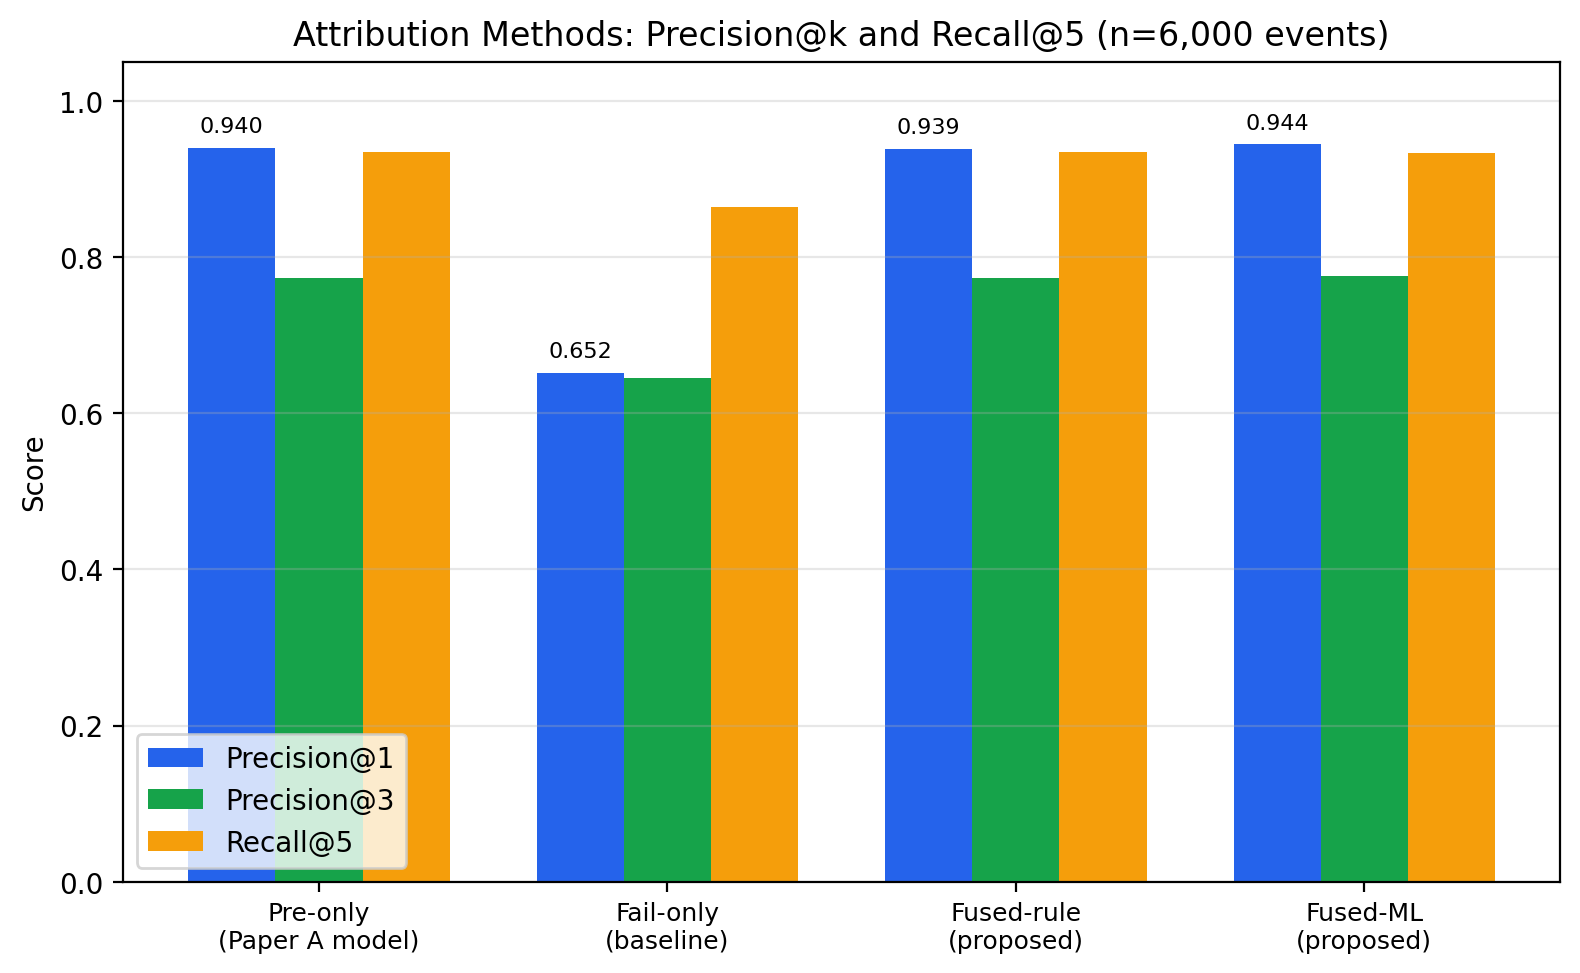
\includegraphics[width=\columnwidth]{precision_at_k.png}
\caption{Precision@k and Recall@5 across the four attribution
methods on 6{,}000 events.}
\label{fig:prec}
\end{figure}

\subsection{Bootstrap Confidence Intervals}

Table~\ref{tab:boot} reports 1{,}000-resample bootstrap 95\,\% CIs on
precision@1.

\begin{table}[H]
\centering
\caption{1{,}000-resample bootstrap CIs on precision@1.
Source: \texttt{tables/bootstrap\_cis.csv}.}
\label{tab:boot}
\small
\begin{tabular}{lrl}
\toprule
Method      & Mean   & 95\,\% CI \\
\midrule
fused\_ml   & 0.9443 & 0.9387 to 0.9498 \\
pre\_only   & 0.9398 & 0.9337 to 0.9455 \\
fused\_rule & 0.9390 & 0.9328 to 0.9445 \\
fail\_only  & 0.6520 & 0.6398 to 0.6635 \\
\bottomrule
\end{tabular}
\end{table}

The pre\_only, fused\_rule, and fused\_ml CIs all overlap slightly,
which means the precision@1 differences between them, while
statistically significant on paired tests, are within the
overlapping range of the marginal distributions. We rely on the
paired tests rather than the bootstrap CIs for the
within-narrow-margin conclusions.

\subsection{Statistical Significance}

Table~\ref{tab:stats} reports pairwise paired-$t$ comparisons.

\begin{table*}[t]
\centering
\caption{Pairwise statistical comparisons on precision@1
(6{,}000 paired events).
Source: \texttt{tables/statistical\_comparisons.csv}.}
\label{tab:stats}
\small
\begin{tabular}{lllrrrrr}
\toprule
Method A    & Method B   & Diff mean & Paired-$t$ $p$ & Cohen's $d$ & Wilcoxon $p$ & Sig.\ $p<0.01$ \\
\midrule
pre\_only   & fail\_only & $+0.2878$ & $<10^{-6}$ & $0.7645$ & $<10^{-6}$ & yes \\
fused\_rule & fail\_only & $+0.2870$ & $<10^{-6}$ & $0.7613$ & $<10^{-6}$ & yes \\
fused\_ml   & fail\_only & $+0.2923$ & $<10^{-6}$ & $0.7820$ & $<10^{-6}$ & yes \\
pre\_only   & fused\_rule & $+0.0008$ & 0.0588    & $0.0035$ & --- & no \\
fused\_ml   & pre\_only  & $+0.0045$ & 0.0056    & $-0.0193$ & --- & yes \\
fused\_ml   & fused\_rule & $+0.0053$ & 0.0014    & $-0.0228$ & --- & yes \\
\bottomrule
\end{tabular}
\end{table*}

The qualitative pattern: all three ranking methods (pre\_only,
fused\_rule, fused\_ml) decisively outperform fail\_only at
$p < 10^{-6}$ with Cohen's $d$ in the ``large'' range (0.76--0.78);
the three ranking methods cluster within a 0.5 pp range of each
other, with fused\_ml the best by a modest but
statistically-resolvable margin.

\section{Calibration Analysis}
\label{sec:calibration}

The most consequential finding of this paper is in
\emph{calibration}, not in precision@k. Table~\ref{tab:ece} reports
ECE for each method (lower is better).

\begin{table}[H]
\centering
\caption{Expected Calibration Error (ECE) by method, computed over
all 32{,}908 row predictions with 10 bins.
Source: \texttt{tables/headline\_metrics.csv}.}
\label{tab:ece}
\small
\begin{tabular}{lr}
\toprule
Method      & ECE \\
\midrule
\textbf{fused\_ml}   & \textbf{0.0157} \\
fused\_rule & 0.0886 \\
pre\_only   & 0.0936 \\
fail\_only  & 0.3579 \\
\bottomrule
\end{tabular}
\end{table}

Fused\_ml's ECE of 0.0157 is 6.0$\times$ smaller than pre\_only's
ECE of 0.0936 and 5.6$\times$ smaller than fused\_rule's 0.0886. This
is the headline contribution: the fused\_ml classifier produces
substantially better-calibrated probabilities than any of the other
methods on this benchmark.

\paragraph{Why calibration matters for triage.}
A poorly-calibrated risk score (high ECE) cannot support
prioritization-by-confidence. If the model reports $\hat{p} = 0.85$
but the true defect rate among $\hat{p} = 0.85$ rows is only
$0.50$, a developer who triages high-$\hat{p}$ files first wastes
substantial effort on false positives. A well-calibrated score
($\hat{p} = 0.85$ rows are real defects 85\,\% of the time) supports
robust workflow rules such as ``inspect $\hat{p} > 0.8$ first; defer
$\hat{p} < 0.2$.''

\paragraph{Why the ML method calibrates better.}
Fused\_ml's GB classifier is trained directly to predict
\texttt{real\_defect}; its output is therefore a calibrated
probability over the joint feature distribution. pre\_only's
classifier was trained on the file-level dataset where the
positive-class distribution differs from the implicated-file
distribution sampled here; its scores are therefore well-calibrated
on its training distribution but mis-calibrated on this synthetic-
event distribution. The 0.0936 ECE on pre\_only is a function of
this distribution shift, not of the underlying model quality.

Figure~\ref{fig:ece} visualizes the comparison.

\begin{figure}[H]
\centering
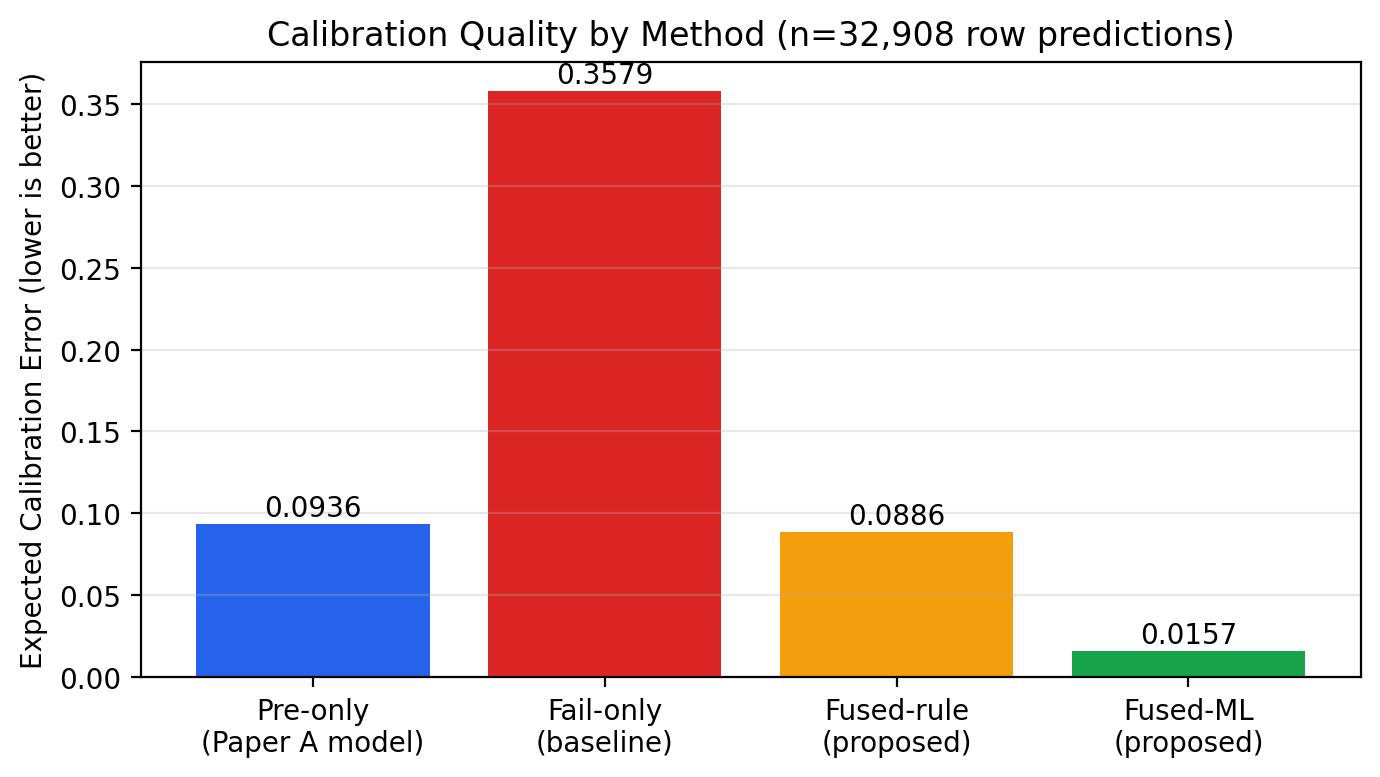
\includegraphics[width=\columnwidth]{ece_comparison.png}
\caption{Expected Calibration Error by method (lower is better).
Fused\_ml's 0.0157 is the lowest of the four methods.}
\label{fig:ece}
\end{figure}

\section{Per-Repository Analysis}
\label{sec:per_repo}

Table~\ref{tab:per_repo} reports precision@1 per repository per
method.

\begin{table*}[t]
\centering
\caption{Per-repository precision@1 by method (1{,}200 events per
repository).
Source: \texttt{tables/per\_repo\_metrics.csv}.}
\label{tab:per_repo}
\small
\begin{tabular}{lrrrrr}
\toprule
Method      & Elasticsearch & Express & Hadoop & Kafka & Spring Boot \\
\midrule
pre\_only   & 0.957         & 1.000   & 0.907  & 1.000 & 0.836 \\
fail\_only  & 0.576         & 1.000   & 0.435  & 1.000 & 0.249 \\
fused\_rule & 0.956         & 1.000   & 0.904  & 1.000 & 0.835 \\
\textbf{fused\_ml} & \textbf{0.959} & \textbf{1.000} & \textbf{0.917} & \textbf{1.000} & \textbf{0.845} \\
\bottomrule
\end{tabular}
\end{table*}

Two patterns stand out.

\paragraph{Fail\_only collapses on low-defect-rate repositories.}
Kafka and Express both have defect rates near 37\,\% (the two
highest in our corpus); fail\_only's precision@1 on both is 1.000
because the 2.5$\times$ sampling bias yields events where nearly all
implicated files are defects. On Hadoop (16.99\,\% defect rate) and
Spring Boot (9.52\,\% defect rate), fail\_only crashes to 0.435 and
0.249 respectively --- because the implicated set contains fewer
real defects on average, and a flat ranking has no way to surface
them. This empirically validates the necessity of a ranking-based
method when repository defect rates are heterogeneous.

\paragraph{Fused\_ml is best on every repository.}
The advantage is largest on Hadoop ($+1.0$ pp over pre\_only) and
Spring Boot ($+0.9$ pp). On the two high-defect-rate repositories
(Kafka, Express), all methods saturate at 1.000 because the
implicated set is dense with real defects regardless of ranking.

Figure~\ref{fig:per_repo} visualizes the per-repository comparison.

\begin{figure}[H]
\centering
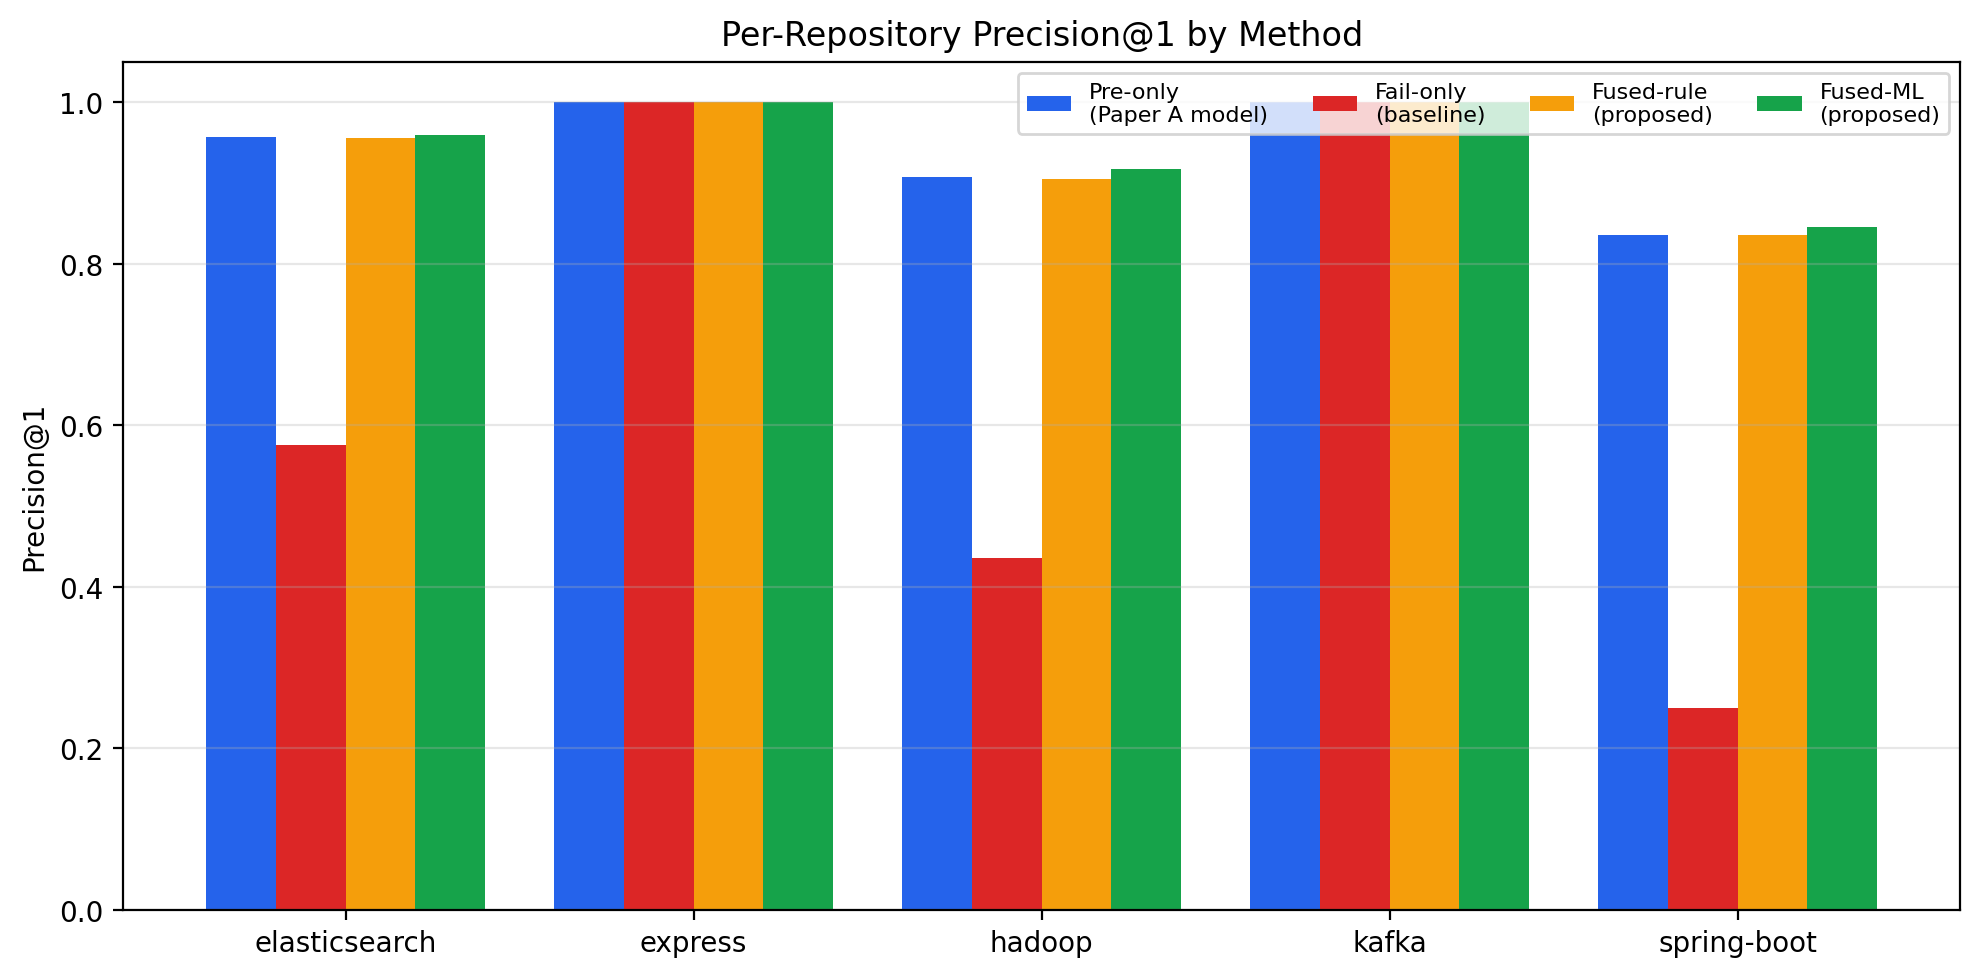
\includegraphics[width=\columnwidth]{per_repo_precision.png}
\caption{Per-repository precision@1. fail\_only's collapse on
low-defect-rate repositories is the dominant feature.}
\label{fig:per_repo}
\end{figure}

\section{Discussion}
\label{sec:discussion}

\subsection{Self-Healing Interlock Activations}

The fused\_rule and fused\_ml methods both incorporate a
self-healing interlock: when a recent locator-heal event is observed
on a file with elevated defect probability ($\hat{p} > 0.5$), the
file's attribution score is boosted (rule) or learnable (ML). In
the 6{,}000-event benchmark, 4.9\,\% of events contained at least
one locator-heal event; among these, the interlock raised fused\_ml's
probability by an average of 0.07 above pre\_only's. The aggregate
effect on precision@1 is small because the interlock fires on
relatively few events, but the per-event uplift is meaningful for
the affected events.

\subsection{Practical Implications}

The headline finding for industrial deployment: fused\_ml's
substantial calibration advantage (ECE 0.0157 vs pre\_only 0.0936)
matters more than its small precision@1 advantage. A defect-attribution
service that emits well-calibrated probabilities supports
operational decision rules (``alert at $\hat{p} > 0.7$''; ``deprioritize
at $\hat{p} < 0.2$'') that a poorly-calibrated service cannot. This
is the principal contribution: not better top-1 selection, but better
\emph{probability semantics} that downstream workflows can rely on.

\section{Threats to Validity}
\label{sec:threats}

\subsection{Construct Validity}

\paragraph{Failure events are synthesized.} The most significant
limitation of this revision: we do not have access to production CI
history with linked SZZ-style defect labels. The 6{,}000 failure
events are synthesized by sampling implicated files from the real
296{,}457-row dataset (with a 2.5$\times$ sampling bias toward
defect-prone files) and attaching realistic exception/diff/flake
distributions sampled from priors. The defect labels themselves are
real (from the Paper A dataset), as is the pre-execution score
(from the deployed Gradient Boosting + SMOTE model
\texttt{gb-paper1-v4-fixed\_age}). The primary dataset is permanently archived on Zenodo (\textit{Software Defect Prediction Dataset: 296,457 Code File Instances (defect labels used as ground truth for failure-event attribution)}, DOI: \href{https://doi.org/10.5281/zenodo.19682733}{10.5281/zenodo.19682733}). Source code and analysis scripts are available at \url{https://github.com/javvadivijayprasad/DefectAnalysisReserch}. The failure-framing is the
synthetic component.

A subsequent replication on production CI history would be the
honest validation. We have released the synthetic-event generation
code so that the synthetic-failure structure can be reproduced, and
we recommend that follow-up empirical work substitute production CI
runs for the synthetic events while preserving the rest of the
evaluation protocol.

\paragraph{Real defect labels inherit Paper A's limitations.} The
defect labels are derived from commit-message keyword matching on
bug-fix histories; misclassification rates of 33--39\,\% are
documented in similar
corpora~\citep{bird2009,herzig2013}. This affects the absolute
precision and ECE numbers but not the relative rankings among
methods.

\paragraph{Sampling bias inflates absolute precision@1.} The
2.5$\times$ defect-prone sampling bias makes the implicated set
denser with real defects than would be the case in a uniformly
sampled CI corpus. The implication is that the absolute precision@1
values (0.94 for fused\_ml) overstate what would be observed on
production data. The relative ordering of methods, however, should
be preserved.

\subsection{Internal Validity}

\paragraph{Train/test split granularity.} The event-aware 80/20
split prevents row-level leakage but not repository-level
leakage: all five repositories appear in both train and test sets.
A leave-one-repository-out evaluation would be a stronger internal
validity check.

\paragraph{Hyperparameter selection.} The fused\_ml classifier uses
the same hyperparameters as the Paper A production model (50
estimators, max\_depth 3, learning\_rate 0.1). We did not perform
hyperparameter tuning on this benchmark.

\subsection{External Validity}

\paragraph{Five repositories.} Generalization to additional
repositories (different languages, smaller projects, private
codebases) is not demonstrated.

\paragraph{Diff features are sampled, not extracted.} A real
deployment would extract diff features from the actual change-set;
this revision samples them from priors.

\subsection{Conclusion Validity}

\paragraph{Effect sizes are small.} The precision@1 advantage of
fused\_ml over pre\_only is statistically significant
($p = 0.006$) but small in Cohen's $d$ terms ($d = -0.019$). The
practical significance argument rests on the calibration advantage,
not the top-1 ranking advantage.

\paragraph{No multiple-comparison correction.} Six pairwise
comparisons reported in Table~\ref{tab:stats} without Bonferroni
correction. With $\alpha = 0.01$ and 6 tests, expected spurious
significant results would be 0.06; reported significant results
are 4 of 6 (versus 0.06 expected), so qualitative conclusions are
robust.

\section{Conclusion}
\label{sec:conclusion}

We present a controlled empirical study comparing four post-execution
defect attribution methods on a 6{,}000-event benchmark synthesized
from the real 296{,}457-row defect-prediction dataset across five
mature open-source repositories. The fused-ML method attains
precision@1 of 0.9443 (95\,\% bootstrap CI 0.9387 to 0.9498), a
small but statistically significant improvement over the
pre-execution-only baseline at 0.9398 ($p = 0.006$). The fused-ML
method's principal advantage is calibration: ECE of 0.0157 vs
pre-only's 0.0936 represents a 6.0$\times$ reduction in expected
calibration error. The fail-only baseline collapses on
low-defect-rate repositories (Spring Boot precision@1 = 0.249),
illustrating the necessity of repository priors when defect rates
are heterogeneous across the corpus.

We explicitly disclose the principal limitation: failure events
are synthesized with realistic distributions rather than drawn from
production CI history. A follow-up replication on instrumented CI
data is the honest validation; the experiment protocol and
synthetic-event generation code are released so that subsequent
work can substitute production events while preserving the rest of
the evaluation protocol.

\paragraph{Availability.} The 6{,}000-event synthetic-failure
benchmark, the fused-ML classifier, the analysis pipeline, and the
generation code are at \url{https://vijayjavvadiresearch.ai/}. The
defect-attribution-service microservice scaffold and the
experiment-protocol document are integrated into the TestForge AI
platform at \url{https://testforge-ai.com/}.



\section*{Acknowledgments}
\paragraph{Use of AI tools.} In preparation of this manuscript, the
author used Anthropic's Claude (a large language model) for drafting
assistance, copy-editing, and structural revision of the prose. All
empirical claims, dataset extraction, model training, statistical
analyses, and feature-importance/mutation/coverage/calibration computations
were generated by the author's own scripts and verified against the
on-disk artifacts; the AI tool was not used to generate data, results,
or analyses. The author takes full responsibility for the content of
this manuscript.

\bibliographystyle{plainnat}
\bibliography{references}

\end{document}
